\begin{frame}{Overview}
    \begin{center}
        $\O^\star((2 - \varepsilon)^\td)$ for \IS\qquad $\Rightarrow$ \qquad $\O^\star((2 - \varepsilon')^n)$ for SAT
    \end{center}

    \pause

    \vspace{.5cm}

    Given a formula $\phi$:
    \begin{enumerate}
        \item<2-> Build $G = (V, E)$ and $k$ depending on $\phi$ and $\varepsilon$. We want:\begin{itemize}
            \item<3-> $\td(G) \approx n$,
            \item<4-> $\phi \in \text{SAT} \Leftrightarrow (G, k) \in \IS$.
        \end{itemize}
        \item<5-> Run \IS\ for $(G, k)$ in time $\O^\star((2 - \varepsilon)^\td)$.
        \item<6-> Return the same answer for the question "$\phi \in \text{SAT}$?".
        \item<7-> We have an algorithm in $\O^\star((2 - \varepsilon')^n)$ for SAT. Contradicting SETH.
    \end{enumerate}
\end{frame}

\begin{frame}{Preliminaries}
    \begin{itemize}
        \item Choose $p = f(\varepsilon)$ \only<2->{{\color{red}$= 6$}.}
        \item<4-> Cut variables into groups of size at most $\lfloor\log\binom{p}{p/2}\rfloor {\color{red} = 4}$.
    \end{itemize}

    \centering

    \onslide<3->{
\tikzstyle{group} = [draw=red,ultra thick]

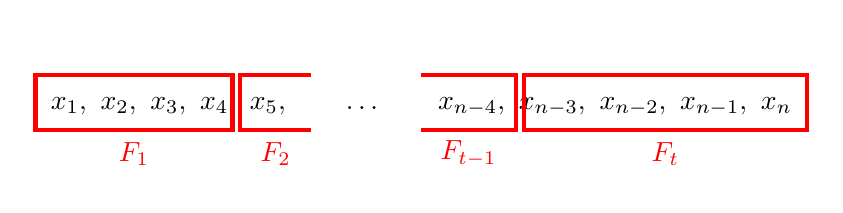
\begin{tikzpicture}
    \path (-5, -1) -- (5, -1) -- (5, 1) -- (-5, 1) -- cycle;
    \node[] at (0,0) {$x_1,\ x_2,\ x_3,\ x_4,\ x_5, \qquad \dots \qquad x_{n-4},\ x_{n-3},\ x_{n-2},\ x_{n-1},\ x_n$};

    \draw<4-> [style=group] (-4.9,-.3) -- (-2.4,-.3) -- (-2.4, .4) -- (-4.9, .4) -- cycle;
    \draw<4-> [style=group] (-1.4, .4) -- (-2.3, .4) -- (-2.3,-.3) -- (-1.4,-.3);
    \draw<4-> [style=group] (0, .4) -- (1.2, .4) -- (1.2,-.3) -- (0,-.3);
    \draw<4-> [style=group] (4.9, -.3) -- (1.3,-.3) -- (1.3, .4) -- (4.9, .4) -- cycle;

    \node<4-> at (-3.65, -.6) {\color{red}$F_1$};
    \node<4-> at (-1.85, -.6) {\color{red}$F_2$};
    \node<4-> at (.6, -.6) {\color{red}$F_{t-1}$};
    \node<4-> at (3.1, -.6) {\color{red}$F_t$};
\end{tikzpicture}}
\end{frame}

\begin{frame}
    \frametitle{Group gadget}
    \centering
    \tikzstyle{vertex} = [draw=black,fill=black,circle,inner sep=0pt,minimum size=3pt]
\tikzstyle{chosen} = [draw=black,fill=red,circle,inner sep=0pt,minimum size=5pt]
\tikzstyle{edgeA} = [draw=black]
\tikzstyle{edgeClique} = [draw=red, line width=3pt]
\tikzstyle{comp} = [draw=black,fill=white,circle,inner sep=0pt,minimum size=20pt]

\begin{tikzpicture}[scale=0.6]
    \path (-1,-3) -- (15,-3) -- (15,8) -- (-1,8) -- cycle;

    \foreach \x [evaluate=\x as \pos using \x - 1] in {1,...,6}{
        \coordinate (I\x) at (0,\pos);
    }
    \foreach \x [evaluate=\x as \pos using 2.5 + \x*0.75] in {1,...,4}{
        \coordinate (A\x) at (2,\pos);
    }
    \foreach \x [evaluate=\x as \pos using -1.5 + \x*0.75] in {1,...,4}{
        \coordinate (B\x) at (2,\pos);
    }

    \foreach \x in {1,...,6}{
        \node [style=vertex] at (I\x) {};
    }
    \foreach \x in {1,...,4}{
        \node<8-10> [style=vertex] at (A\x) {};
    }
    \foreach \x in {1,...,4}{
        \node<12-13> [style=vertex] at (B\x) {};
    }

    \foreach \x in {1,...,4}{
        \coordinate (X\x) at ($(\x, 0) + (8, 7)$);
        \coordinate (VX\x) at ($(\x, 0) + (8, 6)$);
        \node<-5> at (X\x) {$x_\x$};
    }

    \node<2> at (VX1) {\textbf{\color{green}T}};
    \node<2-3> at (VX2) {\textbf{\color{green}T}};
    \node<2,4-5> at (VX3) {\textbf{\color{green}T}};
    \node<2,4-5> at (VX4) {\textbf{\color{green}T}};

    \node<3-5> at (VX1) {\textbf{\color{red}F}};
    \node<4,5> at (VX2) {\textbf{\color{red}F}};
    \node<3> at (VX3) {\textbf{\color{red}F}};
    \node<3> at (VX4) {\textbf{\color{red}F}};

    \foreach \y in {4,5,6}{
        \node<2> [style=chosen] at (I\y) {};
    }
    \foreach \y in {2,3,5}{
        \node<3> [style=chosen] at (I\y) {};
    }
    \foreach \y in {1,2,6}{
        \node<4-5> [style=chosen] at (I\y) {};
    }

    \node<5> at (10.5,4) {$2^{\lfloor\log\binom{p}{p/2}\rfloor} \leq \binom{p}{p/2}$};

    \draw<-5,14-> [orange, line width=2pt] (0,2.5) ellipse (.8cm and 3.5cm);
    \node<-5,14-> at (0,6.5) {\color{orange}$|I| = p$};

    \foreach \y in {4,5,6}{
        \foreach \x in {1,...,4}{
            \draw<8-10> [style=edgeA] (I\y) -- (A\x);
        }
    }
    \foreach \y in {1,2,3}{
        \node<10,17-18> [style=chosen] at (I\y) {};
    }
    \foreach \x in {1,...,4}{
        \node<10> [style=chosen] at (A\x) {};
    }

    \node<7-10> at (0,6) {\color{blue}$\overline{A}_1$};
    \draw<7-10> [blue, line width=2pt] (0,4) ellipse (.5cm and 1.4cm);
    \node<9-10> at (2,7) {\color{blue}$A'_1$};
    \draw<9-10> [blue, line width=2pt] (2,4.3) ellipse (.6cm and 2cm);
    \node<6-10> at (0,-1) {\color{blue}$A_1$};
    \draw<6-10> [blue, line width=2pt] (0,1) ellipse (.5cm and 1.4cm);

    \foreach \y in {2,3,5}{
        \foreach \x in {1,...,4}{
            \draw<12-13> [style=edgeA] (I\y) -- (B\x);
        }
    }
    \foreach \y in {1,4,6}{
        \node<13> [style=chosen] at (I\y) {};
    }
    \foreach \x in {1,...,4}{
        \node<13> [style=chosen] at (B\x) {};
    }

    % TODO faire le vrai ensemble en bleu
    \draw<11-13> [blue, line width=2pt] (2,.3) ellipse (.6cm and 2cm);
    \node<11-13> at (2,3) {\color{blue}$A_2$};

    \foreach \x in {1,2,...,6}{
        \coordinate (C\x) at ($(6.5,2.5) + (180 - \x*360/7: 4cm)$);
        \node<14-> at ($(6.5,2.5) + (180 - \x*360/7: 5.2cm)$) {\color{blue}$A'_\x$};
    }
    \foreach \x in {1,...,5}{
        \foreach \y in {\x,...,6}{
            \draw<16-> [style=edgeClique] (C\x) -- (C\y);
        }
    }
    \foreach \x in {1,2,...,6}{
        \node<14-> [style=comp] at (C\x) {};
        \foreach \a [count=\i] in {-.2,.2}{
            \foreach \b [count=\j] in {-.2,.2}{
                \coordinate (p\x\i\j) at ($(C\x) + (\a, \b)$);
                \node<14-> [style=vertex] at (p\x\i\j) {};
                \node<15> [style=chosen] at (p\x\i\j) {};
            }
        }
    }
    \foreach \y in {4,5,6}{
        \foreach \i in {1,2}{
            \foreach \j in {1,2}{
                \draw<14-> [style=edgeA,dashed] (I\y) -- (p1\i\j);
            }
        }
    }
    \foreach \i in {1,2}{
        \foreach \j in {1,2}{
            \node<17-18> [style=chosen] at (p1\i\j) {};
        }
    }

    \node<18>  at (11.5, -2) {\#};
    \node<18> [style=chosen] at (12, -2) {};
    \node<18>  at (13.5, -2) {$= p + 1$};
\end{tikzpicture}
\end{frame}

\begin{frame}{Clause gadget}
    \centering
    \tikzstyle{vertex} = [draw=black,fill=black,circle,inner sep=0pt,minimum size=3pt]
\tikzstyle{chosen} = [draw=black,fill=red,circle,inner sep=0pt,minimum size=5pt]
\tikzstyle{edgeI} = [draw=black]
\tikzstyle{edgeTree} = [draw=black]
\tikzstyle{comp} = [draw=black,fill=white,circle,inner sep=0pt,minimum size=20pt]
\tikzstyle{cliqueS} = [blue, line width=2pt, fill=blue!30]
\tikzstyle{cliqueT} = [green, line width=2pt, fill=green!30]

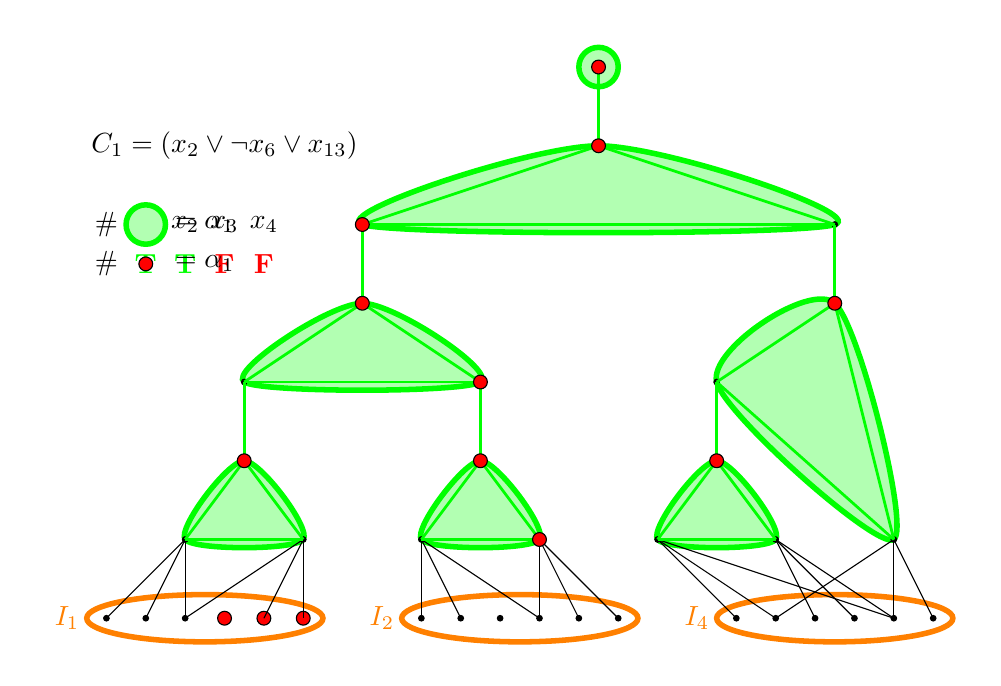
\begin{tikzpicture}[scale=0.5]
    \path (-1,-1) -- (23,-1) -- (23,15) -- (-1,15) -- cycle;

    \node<-23> at (4, 12) {$C_1 = (x_2 \lor \lnot x_6 \lor x_{13})$};

    \foreach \x in {1,...,4}{
        \coordinate (X\x) at (\x + 1, 10);
        \coordinate (VX\x) at (\x + 1, 9);
        \node<3-5> at (X\x) {$x_\x$};
    }

    \node<3-5> at (VX1) {\textbf{\color{green}T}};
    \node<3-5> at (VX2) {\textbf{\color{green}T}};
    \node<3-5> at (VX3) {\textbf{\color{red}F}};
    \node<3-5> at (VX4) {\textbf{\color{red}F}};

    \foreach \n in {0,...,2}{
        \foreach \x in {1,...,6}{
            \coordinate (N\n\x) at (8*\n + \x, 0);
            \node<2->[style=vertex] at (N\n\x) {};
        }
    }

    \draw<2-> [orange, line width=2pt] (3.5, 0) ellipse (3cm and .6cm);
    \node<2-> at (0,0) {\color{orange}$I_1$};
    \draw<2-> [orange, line width=2pt] (11.5, 0) ellipse (3cm and .6cm);
    \node<2-> at (8,0) {\color{orange}$I_2$};
    \draw<2-> [orange, line width=2pt] (19.5, 0) ellipse (3cm and .6cm);
    \node<2-> at (16,0) {\color{orange}$I_4$};

    \foreach \x in {1,...,7}{
        \coordinate (T\x) at (3*\x, 2);
    }
    \foreach \x in {1,...,3}{
        \coordinate (T1\x) at (6*\x - 1.5, 4);
        \coordinate (T2\x) at (6*\x - 1.5, 6);
    }
    \foreach \x in {1,...,2}{
        \coordinate(T3\x) at (12*\x - 4.5, 8);
        \coordinate(T4\x) at (12*\x - 4.5, 10);
    }
    \coordinate (T51) at (13.5, 12);
    \coordinate (T61) at (13.5, 14);

    % \draw<15> [style=cliqueS] ($(T11)!0.5!(T21)$) ellipse (.6cm and 1.5cm);
    % \draw<15> [style=cliqueS] ($(T12)!0.5!(T22)$) ellipse (.6cm and 1.5cm);
    % \draw<15> [style=cliqueS] ($(T13)!0.5!(T23)$) ellipse (.6cm and 1.5cm);
    % \draw<15> [style=cliqueS] ($(T31)!0.5!(T41)$) ellipse (.6cm and 1.5cm);
    % \draw<15> [style=cliqueS] ($(T32)!0.5!(T42)$) ellipse (.6cm and 1.5cm);
    % \draw<15> [style=cliqueS] ($(T51)!0.5!(T61)$) ellipse (.6cm and 1.5cm);
    
    \draw<15-> [style=cliqueT] plot [smooth cycle] coordinates {(T1) (T2) (T11)};
    \draw<15-> [style=cliqueT] plot [smooth cycle] coordinates {(T3) (T4) (T12)};
    \draw<15-> [style=cliqueT] plot [smooth cycle] coordinates {(T5) (T6) (T13)};
    \draw<15-> [style=cliqueT] plot [smooth cycle] coordinates {(T21) (T22) (T31)};
    \draw<15-> [style=cliqueT] plot [smooth cycle] coordinates {(T7) (T23) (T32)};
    \draw<15-> [style=cliqueT] plot [smooth cycle] coordinates {(T41) (T42) (T51)};
    \draw<15-> [style=cliqueT] (T61) ellipse (.5cm and .5cm);

    \node<15-23> at (1, 10) {\#};
    \draw<15-23> [style=cliqueT] (2,10) ellipse (.5cm and .5cm);
    \node<15-23> at (3.5, 10) {$= \alpha_1$};

    \node<4->[style=vertex] at (T1) {};
    \foreach \x in {4,5,6} {
        \node<3-5>[style=chosen] at (N0\x) {};
    }
    \foreach \x in {1,2,3} {
        \draw<5->[style=edgeI] (N0\x) -- (T1);
    }
    \node<6->[style=vertex] at (T2) {};
    \foreach \x in {3,5,6} {
        \draw<6->[style=edgeI] (N0\x) -- (T2);
    }
    \node<6->[style=vertex] at (T3) {};
    \foreach \x in {1,2,4} {
        \draw<6->[style=edgeI] (N1\x) -- (T3);
    }
    \node<6->[style=vertex] at (T4) {};
    \foreach \x in {4,5,6} {
        \draw<6->[style=edgeI] (N1\x) -- (T4);
    }
    \node<6->[style=vertex] at (T5) {};
    \foreach \x in {1,2,5} {
        \draw<6->[style=edgeI] (N2\x) -- (T5);
    }
    \node<6->[style=vertex] at (T6) {};
    \foreach \x in {3,4,5} {
        \draw<6->[style=edgeI] (N2\x) -- (T6);
    }
    \node<6->[style=vertex] at (T7) {};
    \foreach \x in {2,5,6} {
        \draw<6->[style=edgeI] (N2\x) -- (T7);
    }

    \node<8-> [style=vertex] at (T11) {};
    \node<9-> [style=vertex] at (T21) {};
    \draw<7-> [style=edgeTree] (T1) -- (T2);
    \draw<8-> [style=edgeTree] (T1) -- (T11);
    \draw<8-> [style=edgeTree] (T2) -- (T11);
    \draw<9-> [style=edgeTree] (T11) -- (T21);

    \node<10-> [style=vertex] at (T12) {};
    \node<10-> [style=vertex] at (T22) {};
    \draw<10-> [style=edgeTree] (T3) -- (T4);
    \draw<10-> [style=edgeTree] (T3) -- (T12);
    \draw<10-> [style=edgeTree] (T4) -- (T12);
    \draw<10-> [style=edgeTree] (T12) -- (T22);

    \node<11-> [style=vertex] at (T13) {};
    \node<11-> [style=vertex] at (T23) {};
    \draw<11-> [style=edgeTree] (T5) -- (T6);
    \draw<11-> [style=edgeTree] (T5) -- (T13);
    \draw<11-> [style=edgeTree] (T6) -- (T13);
    \draw<11-> [style=edgeTree] (T13) -- (T23);

    \node<12-> [style=vertex] at (T32) {};
    \node<12-> [style=vertex] at (T42) {};
    \draw<12-> [style=edgeTree] (T7) -- (T23);
    \draw<12-> [style=edgeTree] (T7) -- (T32);
    \draw<12-> [style=edgeTree] (T23) -- (T32);
    \draw<12-> [style=edgeTree] (T32) -- (T42);

    \node<13-> [style=vertex] at (T31) {};
    \node<13-> [style=vertex] at (T41) {};
    \draw<13-> [style=edgeTree] (T21) -- (T22);
    \draw<13-> [style=edgeTree] (T21) -- (T31);
    \draw<13-> [style=edgeTree] (T22) -- (T31);
    \draw<13-> [style=edgeTree] (T31) -- (T41);

    \node<14-> [style=vertex] at (T51) {};
    \node<14-> [style=vertex] at (T61) {};
    \draw<14-> [style=edgeTree] (T41) -- (T42);
    \draw<14-> [style=edgeTree] (T41) -- (T51);
    \draw<14-> [style=edgeTree] (T42) -- (T51);
    \draw<14-> [style=edgeTree] (T51) -- (T61);

    \node<16-23>[style=chosen] at (T11) {};
    \node<16-18>[style=chosen] at (T12) {};
    \node<16-23>[style=chosen] at (T13) {};
    \node<17-19>[style=chosen] at (T31) {};
    \node<17-23>[style=chosen] at (T32) {};
    \node<18-20>[style=chosen] at (T51) {};

    \node<19-23>[style=chosen] at (T4) {};
    \node<20-23>[style=chosen] at (T22) {};
    \node<21-23>[style=chosen] at (T41) {};
    \node<22-23>[style=chosen] at (T61) {};

    \node<23>  at (1, 9) {\#};
    \node<23> [style=chosen] at (2, 9) {};
    \node<23>  at (3.5, 9) {$= \alpha_1$};
\end{tikzpicture}
\end{frame}

\begin{frame}{Equivalence}
    \centering
    \begin{itemize}
        \item Let $G$ be the combination of group gadgets and clause gadgets.
        \item Let $k = t(p+1)+ \sum_{i = 1}^m \alpha_i$
    \end{itemize}

    \vspace{1cm}

    $(G, k) \in \IS \Leftrightarrow \phi \in \text{SAT}$
\end{frame}

\begin{frame}<0>[label=proof]
    \frametitle{Treedepth of $G$}
    \begin{tikzpicture}
        % \path[draw=red] (-6, -5) -- (7, -5) -- (7, 2) -- (-6, 2) -- cycle;
        \onslide<25-26>{
        \node at (0,1.5) {
            \scalebox{.5}{
                \tikzstyle{vertex} = [draw=black,fill=black,circle,inner sep=0pt,minimum size=3pt]
\tikzstyle{chosen} = [draw=black,fill=red,circle,inner sep=0pt,minimum size=5pt]
\tikzstyle{edgeA} = [draw=black]
\tikzstyle{edgeClique} = [draw=red, line width=3pt]
\tikzstyle{comp} = [draw=black,fill=white,circle,inner sep=0pt,minimum size=20pt]

\begin{tikzpicture}[scale=0.6]
    \path (-1,-3) -- (15,-3) -- (15,8) -- (-1,8) -- cycle;

    \foreach \x [evaluate=\x as \pos using \x - 1] in {1,...,6}{
        \coordinate (I\x) at (0,\pos);
    }
    \foreach \x [evaluate=\x as \pos using 2.5 + \x*0.75] in {1,...,4}{
        \coordinate (A\x) at (2,\pos);
    }
    \foreach \x [evaluate=\x as \pos using -1.5 + \x*0.75] in {1,...,4}{
        \coordinate (B\x) at (2,\pos);
    }

    \foreach \x in {1,...,6}{
        \node [style=vertex] at (I\x) {};
    }
    \foreach \x in {1,...,4}{
        \node<8-10> [style=vertex] at (A\x) {};
    }
    \foreach \x in {1,...,4}{
        \node<12-13> [style=vertex] at (B\x) {};
    }

    \foreach \x in {1,...,4}{
        \coordinate (X\x) at ($(\x, 0) + (8, 7)$);
        \coordinate (VX\x) at ($(\x, 0) + (8, 6)$);
        \node<-5> at (X\x) {$x_\x$};
    }

    \node<2> at (VX1) {\textbf{\color{green}T}};
    \node<2-3> at (VX2) {\textbf{\color{green}T}};
    \node<2,4-5> at (VX3) {\textbf{\color{green}T}};
    \node<2,4-5> at (VX4) {\textbf{\color{green}T}};

    \node<3-5> at (VX1) {\textbf{\color{red}F}};
    \node<4,5> at (VX2) {\textbf{\color{red}F}};
    \node<3> at (VX3) {\textbf{\color{red}F}};
    \node<3> at (VX4) {\textbf{\color{red}F}};

    \foreach \y in {4,5,6}{
        \node<2> [style=chosen] at (I\y) {};
    }
    \foreach \y in {2,3,5}{
        \node<3> [style=chosen] at (I\y) {};
    }
    \foreach \y in {1,2,6}{
        \node<4-5> [style=chosen] at (I\y) {};
    }

    \node<5> at (10.5,4) {$2^{\lfloor\log\binom{p}{p/2}\rfloor} \leq \binom{p}{p/2}$};

    \draw<-5,14-> [orange, line width=2pt] (0,2.5) ellipse (.8cm and 3.5cm);
    \node<-5,14-> at (0,6.5) {\color{orange}$|I| = p$};

    \foreach \y in {4,5,6}{
        \foreach \x in {1,...,4}{
            \draw<8-10> [style=edgeA] (I\y) -- (A\x);
        }
    }
    \foreach \y in {1,2,3}{
        \node<10,17-18> [style=chosen] at (I\y) {};
    }
    \foreach \x in {1,...,4}{
        \node<10> [style=chosen] at (A\x) {};
    }

    \node<7-10> at (0,6) {\color{blue}$\overline{A}_1$};
    \draw<7-10> [blue, line width=2pt] (0,4) ellipse (.5cm and 1.4cm);
    \node<9-10> at (2,7) {\color{blue}$A'_1$};
    \draw<9-10> [blue, line width=2pt] (2,4.3) ellipse (.6cm and 2cm);
    \node<6-10> at (0,-1) {\color{blue}$A_1$};
    \draw<6-10> [blue, line width=2pt] (0,1) ellipse (.5cm and 1.4cm);

    \foreach \y in {2,3,5}{
        \foreach \x in {1,...,4}{
            \draw<12-13> [style=edgeA] (I\y) -- (B\x);
        }
    }
    \foreach \y in {1,4,6}{
        \node<13> [style=chosen] at (I\y) {};
    }
    \foreach \x in {1,...,4}{
        \node<13> [style=chosen] at (B\x) {};
    }

    % TODO faire le vrai ensemble en bleu
    \draw<11-13> [blue, line width=2pt] (2,.3) ellipse (.6cm and 2cm);
    \node<11-13> at (2,3) {\color{blue}$A_2$};

    \foreach \x in {1,2,...,6}{
        \coordinate (C\x) at ($(6.5,2.5) + (180 - \x*360/7: 4cm)$);
        \node<14-> at ($(6.5,2.5) + (180 - \x*360/7: 5.2cm)$) {\color{blue}$A'_\x$};
    }
    \foreach \x in {1,...,5}{
        \foreach \y in {\x,...,6}{
            \draw<16-> [style=edgeClique] (C\x) -- (C\y);
        }
    }
    \foreach \x in {1,2,...,6}{
        \node<14-> [style=comp] at (C\x) {};
        \foreach \a [count=\i] in {-.2,.2}{
            \foreach \b [count=\j] in {-.2,.2}{
                \coordinate (p\x\i\j) at ($(C\x) + (\a, \b)$);
                \node<14-> [style=vertex] at (p\x\i\j) {};
                \node<15> [style=chosen] at (p\x\i\j) {};
            }
        }
    }
    \foreach \y in {4,5,6}{
        \foreach \i in {1,2}{
            \foreach \j in {1,2}{
                \draw<14-> [style=edgeA,dashed] (I\y) -- (p1\i\j);
            }
        }
    }
    \foreach \i in {1,2}{
        \foreach \j in {1,2}{
            \node<17-18> [style=chosen] at (p1\i\j) {};
        }
    }

    \node<18>  at (11.5, -2) {\#};
    \node<18> [style=chosen] at (12, -2) {};
    \node<18>  at (13.5, -2) {$= p + 1$};
\end{tikzpicture}
            }
        };
        }
        \onslide<27-29>{
        \node at (0,1.5) {
            \scalebox{.5}{
                \tikzstyle{vertex} = [draw=black,fill=black,circle,inner sep=0pt,minimum size=3pt]
\tikzstyle{chosen} = [draw=black,fill=red,circle,inner sep=0pt,minimum size=5pt]
\tikzstyle{edgeI} = [draw=black]
\tikzstyle{edgeTree} = [draw=black]
\tikzstyle{comp} = [draw=black,fill=white,circle,inner sep=0pt,minimum size=20pt]
\tikzstyle{cliqueS} = [blue, line width=2pt, fill=blue!30]
\tikzstyle{cliqueT} = [green, line width=2pt, fill=green!30]

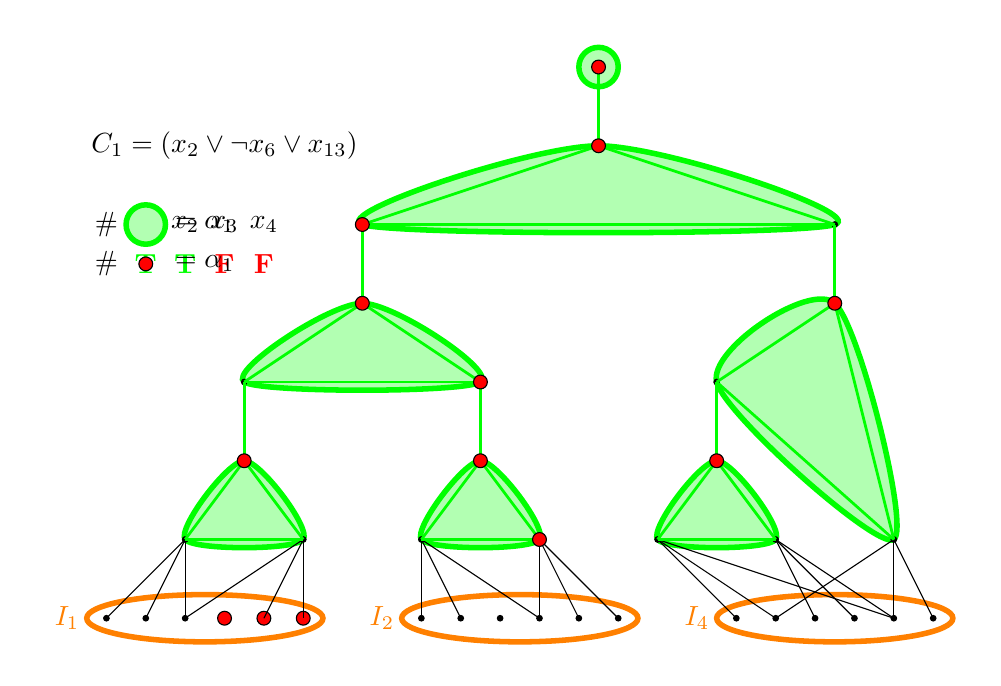
\begin{tikzpicture}[scale=0.5]
    \path (-1,-1) -- (23,-1) -- (23,15) -- (-1,15) -- cycle;

    \node<-23> at (4, 12) {$C_1 = (x_2 \lor \lnot x_6 \lor x_{13})$};

    \foreach \x in {1,...,4}{
        \coordinate (X\x) at (\x + 1, 10);
        \coordinate (VX\x) at (\x + 1, 9);
        \node<3-5> at (X\x) {$x_\x$};
    }

    \node<3-5> at (VX1) {\textbf{\color{green}T}};
    \node<3-5> at (VX2) {\textbf{\color{green}T}};
    \node<3-5> at (VX3) {\textbf{\color{red}F}};
    \node<3-5> at (VX4) {\textbf{\color{red}F}};

    \foreach \n in {0,...,2}{
        \foreach \x in {1,...,6}{
            \coordinate (N\n\x) at (8*\n + \x, 0);
            \node<2->[style=vertex] at (N\n\x) {};
        }
    }

    \draw<2-> [orange, line width=2pt] (3.5, 0) ellipse (3cm and .6cm);
    \node<2-> at (0,0) {\color{orange}$I_1$};
    \draw<2-> [orange, line width=2pt] (11.5, 0) ellipse (3cm and .6cm);
    \node<2-> at (8,0) {\color{orange}$I_2$};
    \draw<2-> [orange, line width=2pt] (19.5, 0) ellipse (3cm and .6cm);
    \node<2-> at (16,0) {\color{orange}$I_4$};

    \foreach \x in {1,...,7}{
        \coordinate (T\x) at (3*\x, 2);
    }
    \foreach \x in {1,...,3}{
        \coordinate (T1\x) at (6*\x - 1.5, 4);
        \coordinate (T2\x) at (6*\x - 1.5, 6);
    }
    \foreach \x in {1,...,2}{
        \coordinate(T3\x) at (12*\x - 4.5, 8);
        \coordinate(T4\x) at (12*\x - 4.5, 10);
    }
    \coordinate (T51) at (13.5, 12);
    \coordinate (T61) at (13.5, 14);

    % \draw<15> [style=cliqueS] ($(T11)!0.5!(T21)$) ellipse (.6cm and 1.5cm);
    % \draw<15> [style=cliqueS] ($(T12)!0.5!(T22)$) ellipse (.6cm and 1.5cm);
    % \draw<15> [style=cliqueS] ($(T13)!0.5!(T23)$) ellipse (.6cm and 1.5cm);
    % \draw<15> [style=cliqueS] ($(T31)!0.5!(T41)$) ellipse (.6cm and 1.5cm);
    % \draw<15> [style=cliqueS] ($(T32)!0.5!(T42)$) ellipse (.6cm and 1.5cm);
    % \draw<15> [style=cliqueS] ($(T51)!0.5!(T61)$) ellipse (.6cm and 1.5cm);
    
    \draw<15-> [style=cliqueT] plot [smooth cycle] coordinates {(T1) (T2) (T11)};
    \draw<15-> [style=cliqueT] plot [smooth cycle] coordinates {(T3) (T4) (T12)};
    \draw<15-> [style=cliqueT] plot [smooth cycle] coordinates {(T5) (T6) (T13)};
    \draw<15-> [style=cliqueT] plot [smooth cycle] coordinates {(T21) (T22) (T31)};
    \draw<15-> [style=cliqueT] plot [smooth cycle] coordinates {(T7) (T23) (T32)};
    \draw<15-> [style=cliqueT] plot [smooth cycle] coordinates {(T41) (T42) (T51)};
    \draw<15-> [style=cliqueT] (T61) ellipse (.5cm and .5cm);

    \node<15-23> at (1, 10) {\#};
    \draw<15-23> [style=cliqueT] (2,10) ellipse (.5cm and .5cm);
    \node<15-23> at (3.5, 10) {$= \alpha_1$};

    \node<4->[style=vertex] at (T1) {};
    \foreach \x in {4,5,6} {
        \node<3-5>[style=chosen] at (N0\x) {};
    }
    \foreach \x in {1,2,3} {
        \draw<5->[style=edgeI] (N0\x) -- (T1);
    }
    \node<6->[style=vertex] at (T2) {};
    \foreach \x in {3,5,6} {
        \draw<6->[style=edgeI] (N0\x) -- (T2);
    }
    \node<6->[style=vertex] at (T3) {};
    \foreach \x in {1,2,4} {
        \draw<6->[style=edgeI] (N1\x) -- (T3);
    }
    \node<6->[style=vertex] at (T4) {};
    \foreach \x in {4,5,6} {
        \draw<6->[style=edgeI] (N1\x) -- (T4);
    }
    \node<6->[style=vertex] at (T5) {};
    \foreach \x in {1,2,5} {
        \draw<6->[style=edgeI] (N2\x) -- (T5);
    }
    \node<6->[style=vertex] at (T6) {};
    \foreach \x in {3,4,5} {
        \draw<6->[style=edgeI] (N2\x) -- (T6);
    }
    \node<6->[style=vertex] at (T7) {};
    \foreach \x in {2,5,6} {
        \draw<6->[style=edgeI] (N2\x) -- (T7);
    }

    \node<8-> [style=vertex] at (T11) {};
    \node<9-> [style=vertex] at (T21) {};
    \draw<7-> [style=edgeTree] (T1) -- (T2);
    \draw<8-> [style=edgeTree] (T1) -- (T11);
    \draw<8-> [style=edgeTree] (T2) -- (T11);
    \draw<9-> [style=edgeTree] (T11) -- (T21);

    \node<10-> [style=vertex] at (T12) {};
    \node<10-> [style=vertex] at (T22) {};
    \draw<10-> [style=edgeTree] (T3) -- (T4);
    \draw<10-> [style=edgeTree] (T3) -- (T12);
    \draw<10-> [style=edgeTree] (T4) -- (T12);
    \draw<10-> [style=edgeTree] (T12) -- (T22);

    \node<11-> [style=vertex] at (T13) {};
    \node<11-> [style=vertex] at (T23) {};
    \draw<11-> [style=edgeTree] (T5) -- (T6);
    \draw<11-> [style=edgeTree] (T5) -- (T13);
    \draw<11-> [style=edgeTree] (T6) -- (T13);
    \draw<11-> [style=edgeTree] (T13) -- (T23);

    \node<12-> [style=vertex] at (T32) {};
    \node<12-> [style=vertex] at (T42) {};
    \draw<12-> [style=edgeTree] (T7) -- (T23);
    \draw<12-> [style=edgeTree] (T7) -- (T32);
    \draw<12-> [style=edgeTree] (T23) -- (T32);
    \draw<12-> [style=edgeTree] (T32) -- (T42);

    \node<13-> [style=vertex] at (T31) {};
    \node<13-> [style=vertex] at (T41) {};
    \draw<13-> [style=edgeTree] (T21) -- (T22);
    \draw<13-> [style=edgeTree] (T21) -- (T31);
    \draw<13-> [style=edgeTree] (T22) -- (T31);
    \draw<13-> [style=edgeTree] (T31) -- (T41);

    \node<14-> [style=vertex] at (T51) {};
    \node<14-> [style=vertex] at (T61) {};
    \draw<14-> [style=edgeTree] (T41) -- (T42);
    \draw<14-> [style=edgeTree] (T41) -- (T51);
    \draw<14-> [style=edgeTree] (T42) -- (T51);
    \draw<14-> [style=edgeTree] (T51) -- (T61);

    \node<16-23>[style=chosen] at (T11) {};
    \node<16-18>[style=chosen] at (T12) {};
    \node<16-23>[style=chosen] at (T13) {};
    \node<17-19>[style=chosen] at (T31) {};
    \node<17-23>[style=chosen] at (T32) {};
    \node<18-20>[style=chosen] at (T51) {};

    \node<19-23>[style=chosen] at (T4) {};
    \node<20-23>[style=chosen] at (T22) {};
    \node<21-23>[style=chosen] at (T41) {};
    \node<22-23>[style=chosen] at (T61) {};

    \node<23>  at (1, 9) {\#};
    \node<23> [style=chosen] at (2, 9) {};
    \node<23>  at (3.5, 9) {$= \alpha_1$};
\end{tikzpicture}
            }
        };
        }   
        \node at (3,0) {
            \tikzstyle{vertex} = [draw=black,fill=black,circle,inner sep=0pt,minimum size=2pt]
\tikzstyle{edgeI} = [draw=black]
\tikzstyle{edgeTree} = [draw=green, line width=1pt]
\tikzstyle{I} = [orange,line width=2pt]
\tikzstyle{clause} = [black,line width=2pt]
\tikzstyle{clique} = [blue,line width=2pt]

\begin{tikzpicture}[scale=0.4]
    \draw[style=I] (0,0) rectangle (2,4);
    \foreach \x in {1,...,6}{
        \node[style=vertex] (I1\x) at (1,.25 + .5*\x) {};
    }
    \draw[style=I] (0,7) rectangle (2,11);
    \foreach \x in {1,...,6}{
        \node[style=vertex] (I2\x) at (1,7.25 + .5*\x) {};
    }
    \draw[style=I] (0,12) rectangle (2,16);
    \foreach \x in {1,...,6}{
        \node[style=vertex] (I3\x) at (1,12.25 + .5*\x) {};
    }
    \node at (-1,2) {\color{orange}$I_t$};
    \node at (-1,9) {\color{orange}$I_2$};
    \node at (-1,14) {\color{orange}$I_1$};

    \node[fill=white,circle,minimum size=15pt] (dots) at (1, 5.5) {};
    \node at (1, 5.75) {$\vdots$};

    \draw[style=edgeTree] (I11) -- (I12) -- (I13) -- (I14) -- (I15) -- (I16);
    \draw[style=edgeTree] (I21) -- (I22) -- (I23) -- (I24) -- (I25) -- (I26);
    \draw[style=edgeTree] (I31) -- (I32) -- (I33) -- (I34) -- (I35) -- (I36);
    \draw[style=edgeTree] (I16) -- (dots) -- (I21);
    \draw[style=edgeTree] (I26) -- (I31);

    \foreach \x in {0,...,3}{
        \draw[style=edgeTree] (-3*\x - 2,-1) -- (I11);
        \draw[style=clause] (-3*\x - 3,-3) -- (-3*\x - 2,-1) -- (-3*\x - 1,-3) -- cycle;
    }

    \coordinate (C1) at (3.5, 12);
    \coordinate (C2) at (3.5, 7);
    \coordinate (C3) at (3.5, 0);

    \draw[style=edgeTree] (C1) -- (I31);
    \draw[style=edgeTree] (C2) -- (I21);
    \draw[style=edgeTree] (C3) -- (I11);

    \node [style=vertex] at (C1) {};
    \node [style=vertex] at (C2) {};
    \node [style=vertex] at (C3) {};

    \draw[style=clique] (C1) ellipse (.6cm and 2cm);
    \draw[style=clique] (C2) ellipse (.6cm and 2cm);
    \draw[style=clique] (C3) ellipse (.6cm and 2cm);

    \onslide<30->{\draw[style=I,Latex-Latex] (-5,0) -- (-5, 16) node [midway, left] {\color{orange}$tp$};}
    \onslide<26->{\draw[style=clique,Latex-Latex] (5,-2) -- (5, 2) node [midway, right] {\color{blue}$f_1(p)$};}
    \onslide<28>{\draw[style=clause,Latex-Latex] (-13,-4) -- (-13, 0) node [midway, left] {$\O(\log(t\binom{p}{p/2}))$};}
    \onslide<29->{\draw[style=clause,Latex-Latex] (-13,-4) -- (-13, 0) node [midway, left] {$\O(\log n) + f_2(p)$};}
\end{tikzpicture}
        };
    \end{tikzpicture}
\end{frame}

\againframe<24->{proof}

\begin{frame}{Conclusion of the proof}
    \begin{itemize}
        \item $\td(G) = tp + \O(\log n) + c$
        \item Let $\lambda$ such that $(2 - \varepsilon)^{1 + \lambda} \leq (2 - \varepsilon')$
        \item Choose $p$ such that $p/(p - \frac{1}{2} + \frac{1}{2} \log(\pi p)) \leq 1 + \lambda$
        \item We optain $\O^\star((2 - \varepsilon)^{\td(G)}) \leq \O^\star((2 - \varepsilon')^n)$
    \end{itemize}

    \hfill$\square$
\end{frame}